\subsection{逆向if-conversion}

\textbf{逆向if-conversion(reverse if-conversion,简称RIC)}由Warter在1993您引入,能够将谓词化的语句重新转换成分支语句。Warter最初引入逆向if-conversion是为了利用if-conversion的分支消除功能实现全局调度,后来逆向if-conversion被用来平衡程序中的控制流跟谓词执行。

程序的分支是靠分支语句来实现的,分支语句将代码分割成若干基本块,每个基本块内部代码顺序执行,而分支语句则在基本块之间进行跳转。多条分支最终都汇集到一起是一个非常常见的事情,分支的汇集不需要任何语句的支持,多条路径最终跳转到统一基本块的时候,分支自动就汇集了。然而为了方便,引入\textbf{隐式合并操作(implicit merge operation)}的概念:认为在多条分支合并到的基本块中有一个隐式合并操作,该操作位于基本块中所有语句之前(就好比分支语句位于基本块中所有语句之后)。

类比控制依赖的概念,Warter提出了反控制依赖的概念。

\begin{definition}[支配(dominate)]
设V与W是控制流图G中的节点,如果从START到V的每条路径都包含W,则称V被W支配。
\end{definition}

\begin{definition}[反控制依赖(reverse control dependent)]
设G为控制流图,X以及Y是图中节点,称X反控制依赖于Y当且仅当:
\begin{enumerate}
\item 存在从X到Y的路径P,使得X支配P上除了Y的所有节点。
\item X不支配Y
\end{enumerate}
\end{definition}
类似控制依赖的$CD\left(x\right)$函数,可以为反控制依赖定义$RCD\left(x\right)$函数。该函数的计算算法可以类比控制依赖的计算算法很容易地得到,在此不再赘述。

if-conversion会将程序中的分支删除,并为程序中的每个语句添加谓词,分支语句则被转化成了谓词定义语句。于此类比,隐式合并操作会被转化为\textbf{谓词合并操作(predicate merge operations)}。既然是谓词合并,就要弄清楚到底合并了哪些谓词。

分支语句分出去的分支有true跟false分支的区别,而隐式合并操作合并的分支则存在\textbf{跳转(jump)}与\textbf{非跳转(non-jump)}的区别。虽然在控制流图中,分支都是平等的,但是程序的存放是顺序存放,而指令的执行(如果没有跳转语句的话)也是顺序执行,既然是顺序存放,就要有先有后,这就导致分支汇集的地方,某些汇集来的分支(代码存放在隐式合并操作的正前方)不需要跳转语句直接顺序执行就能达到交汇点,其他的则必须经过跳转从别的地方跳转到此。

\fref{alg:mergedp}计算谓词合并操作合并的谓词,并且将这些为谓词为跳转与非跳转两类,并分别使用$jump\left(t\right)$来表示这两类谓词的集合$no\_jump\left(t\right)$。$jump\left(t\right)$是一个函数,它的定义域是谓词合并操作的集合,对于谓词合并操作t,$jump\left(t\right)$是一个谓词的集合,组成这个集合的谓词被t合并,并且使用集合中谓词的基本块需要经过跳转语句到达谓词合并语句。同理,$no\_jump\left(t\right)$也是一个谓词的集合,使用集合中谓词的基本块要么不需要经过跳转即可顺序执行到达分支合并语句,要么不是谓词合并操作的直接前驱。

\begin{algorithm}[H]
	\label{alg:mergedp}
	\caption{ComputePredicatesToBeMerged}
	\KwIn{控制流图$G\left(N,E,Start\right)$,其中N是G中节点的集合,E是G中边的集合}
	\KwOut{对每个谓词合并操作t,输出$jump\left(t\right)$以及$no\_jump\left(t\right)$}
	\tcc{对于基本块X,记$P\left(X\right)$为X使用的谓词}
	\For{$X\in N$}{
		\For{$t\in RCD\left(X\right)$}{
			\eIf{X不是t的直接后继,或者t在代码存放在X代码的正前方}{
				$no\_jump\left(t\right)=no\_jump\left(t\right)\cup \left\{P\left(X\right)\right\}$\;
			}{
				$jump\left(t\right)=jump\left(t\right)\cup \left\{P\left(X\right)\right\}$\;
			}
		}
	}
\end{algorithm}

逆向if-conversion的算法维护两个数据结构,一个是集合$L$,一个是函数$\rho$。其中$L$表示的是当前所有可能的执行路径的集合,举一个例子方便理解,参见控制流图\fref{fig:pundef},程序刚开始执行的时候,程序只有可能位于A,此时$L=\left\{A\right\}$,在基本块A执行完成以后,程序会进行分支,在编译阶段,无法获知程序会走那条分支,所以此时程序可能位于B或者C,此时$L=\left\{B,C\right\}$。函数$\rho$的被称作\textbf{可行谓词集(allowable predicate set)},它的定义域是$L$,它将$L$中元素$X$映射为一个谓词组成的集合,X被执行当且仅当该集合中所有谓词都为真。

算法从头开始扫描谓词化的程序,针对扫描过程中遇到的每个语句$op$,分情况进行处理:
\begin{itemize}
\item 如果遇到的是谓词定义操作,则在$L$中所有满足$P\left(op\right)\in\rho\left(X\right)$的元素$X$中插入分支语句,并且创建两个新的节点作为分支语句的true跟false分支添加到L中,并设置这两个节点的$\rho$函数为$\rho\left(Succ_t\right)=\rho\left(X\right)\cup true\left(op\right)$,$\rho\left(Succ_f\right)=\rho\left(X\right)\cup false\left(op\right)$,并从$L$中移除该元素。
\item 如果遇到的是谓词合并操作,则为$L$中所有满足$\left[jump\left(op\right)\cup no\_jump\left(op\right)\right]\cap\rho\left(X\right)\neq\varnothing$的元素$X$计算$\rho_{new}\left(X\right)=\rho\left(X\right)-jump\left(op\right)-no\_jump\left(op\right)$,并为所有$jump\left(op\right)\cap\rho\left(X\right)$中的谓词在对应的$X$中插入相应跳转语句, 然后对$\left[jump\left(op\right)\cup no\_jump\left(op\right)\right]\cap\rho\left(X\right)$中的所有谓词搜索与$\rho_{new}\left(X\right)=\rho\left(Y\right)$的元素$Y$,如果找到,则X的后继就是Y,如果没找到,则创建新的后继并且将其可行谓词集设置为$\rho_{new}\left(X\right)$
\item 如果遇到的是普通的谓词化执行语句,则只需在$L$中所有满足$P\left(op\right)\in\rho\left(X\right)$的元素$X$中插入该语句即可。
\end{itemize}

逆向if-conversion的算法如\fref{alg:ric}所示

\begin{algorithm}[H]
	\label{alg:ric}
	\caption{RIC}
	\KwIn{控制流图$G\left(N,E,Start\right)$,其中N是G中节点的集合,E是G中边的集合}
	\KwOut{对每个谓词合并操作t,输出$jump\left(t\right)$以及$no\_jump\left(t\right)$}
	\tcc{对于基本块X,记$P\left(X\right)$为X使用的谓词}
	\For{$X\in N$}{
		\For{$t\in RCD\left(X\right)$}{
			\eIf{X不是t的直接后继,或者t在代码存放在X代码的正前方}{
				$no\_jump\left(t\right)=no\_jump\left(t\right)\cup \left\{P\left(X\right)\right\}$\;
			}{
				$jump\left(t\right)=jump\left(t\right)\cup \left\{P\left(X\right)\right\}$\;
			}
		}
	}
\end{algorithm}
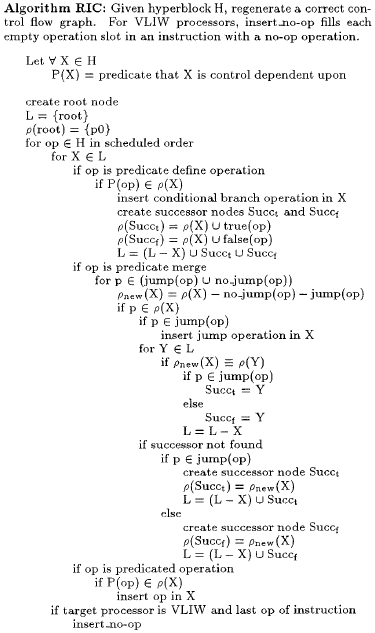
\includegraphics[width=0.9\linewidth]{mechanism/RIC}